\chapter{Исследовательский раздел}

\section{Технические характеристики}

Технические характеристики устройства, на котором выполнялось исследование:
\begin{itemize}[label=---]
	\item операционная система Windows 10 Домашняя 21H2;
	\item оперативная память 12 Гб;
	\item процессор Intel(R) Core(TM) i7-9750H CPU @ 2.6ГГц.
\end{itemize}

Во время проведения замеров времени устройство, помимо исследуемой программы, было нагружено только операционной системой и встроенными приложениями и он было включено в сеть электропитания.

\section{Описание эксперимента и результаты исследования}

Целью эксперимента является изучение влияния индексирования на время обработки запросов к таблицам базы данных.

Эксперимент проводился на таблице ProductDB, содержащих информацию о товарах. Чтобы получить достаточно точное значение, производилось усреднение времени. Количество запусков замера времени для каждого случая --- 10 раз.

\begin{table}[H]
	\begin{center}
		\caption{Замеры времени обработки запросов в зависимости от количеств строк в таблице (с использованием индексирования и без использования индексирования)}
		\begin{tabular}{|c|c|c|}
			\hline
			Количество строк & Без индекса, мс & С индексом, мс \\
			\hline
			1000 & 0.117 & 0.021 \\
			\hline
			1500 & 0.124&0.026\\
			\hline
			2000 & 0.145 & 0.028\\
			\hline
			2500 &0.192 & 0.033\\
			\hline 
		\end{tabular}
		\label{table:db:time}
	\end{center}
\end{table}
\newpage
На рисунке \ref{img:time} приведены графические результаты замеров по времени обработки запросов.
\begin{figure}[ht!]
	\centering
	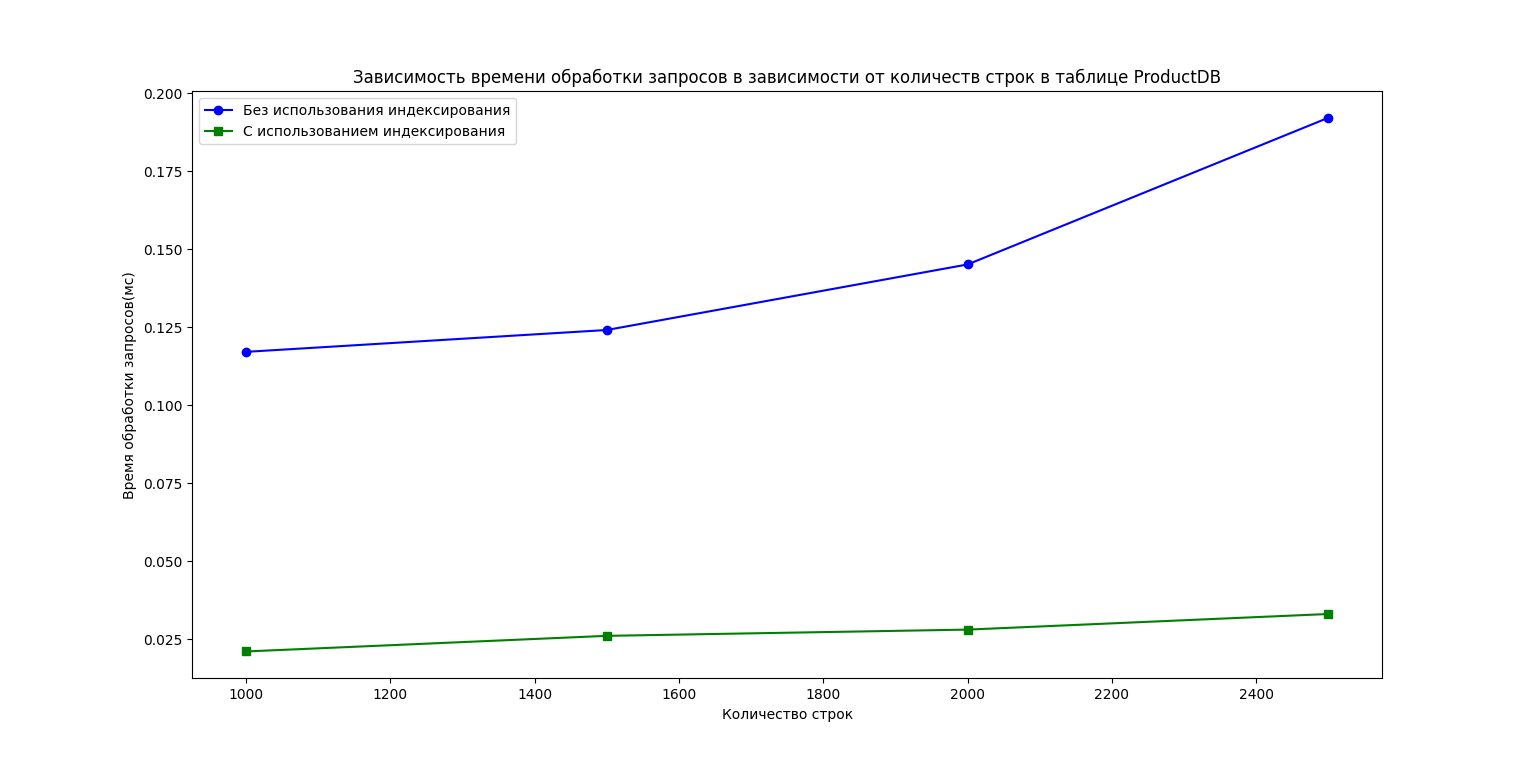
\includegraphics[width=1.1\linewidth]{img/time.png}
	\caption{Сравнение по времени обработки запросов.}
	\label{img:time}
\end{figure}

В результате исследования было выяснено, что без использовании индексирования время обработки запросов медленнее, чем при использовании индексирования, в 5 раз.


\subsection*{Вывод}

Эксперимент показал, что индексация заметно увеличивает скорость выполнения запросов SELECT. Поэтому внедрение индексов в данной системе приведет к улучшению её общей эффективности.